%%%%%%%%%%%%%%%%%%%%%%%%%%%%%%%%%%%%%%%%%%%%%%%%%%%%%%%%%%%%%%%%%%%%%%%%%%%%
%
%  Template code for the Undergraduate Research Scholars thesis program starting, updated by Undergraduate Research Scholars program staff. Version 6.0. Last Updated: Fall 2024
%  Modified by Tawfik Hussein from the template code for TAMU Theses and Dissertations starting Spring 2018, authored by Sean Zachary Roberson. Version 3.17.09.
%
%
%%%%%%%%%%%%%%%%%%%%%%%%%%%%%%%%%%%%%%%%%%%%%%%%%%%%%%%%%%%%%%%%%%%%%%%%%%%%%%%
%%%%%%%%%%%%%%%%%%%%%%%%%%%%%%%%%%%%%%%%%%%%%%%%%%%%%%%%%%%%%%%%%%%%%%%%%%%%%%%
%%                           SECTION III: RESULTS
%%%%%%%%%%%%%%%%%%%%%%%%%%%%%%%%%%%%%%%%%%%%%%%%%%%%%%%%%%%%%%%%%%%%%%%%%%%%%%%

%_________________(0)______________
% Do not modify. This is the page heading

% THIS LINE PUTS "CHAPTER III RESULTS" AT THE TOP OF THE PAGE, BOLD-FACED AND 14-PT
\chapter{RESULTS}

\counterwithout{table}{chapter} % Prevents the table count from resetting in each chapter

%________________(1)_________________
% Modifications needed!

% THIS IS THE SECTION WHERE YOU TYPE IN THE TEXT RELATED TO YOUR RESULTS. NOTICE THE DOUBLE \indent COMMAND THAT PROPERLY INDENTS THE BEGINNING OF EACH PARAGRAPH

% Starting Paragraph One
\indent \indent Paragraph one starts here. If you want to break up your paragraphs into more sections, you can use first order, second order or third order subheadings. 
\\
\indent \indent Feel free to add more Chapters as necessary, but don’t forget to include the Chapter Headings as seen at the top of this page. Also remember that all new Chapters should begin at the top of their own pages and be included in the Table of Contents.
%
%___________________________________________
% Subheading 1 (remove/add as needed)
\vspace{-0.4em} % This line is added to preserve the double-spaced environment since the \section command                      adds an extra space 
\section{Results Subheading 1 (remove/add as needed)}
\vspace{-0.4em} % This line is added to preserve the double-spaced environment since the \section command                      adds an extra space

\indent \indent If you need to enumerate some ideas, the \textit{enumerate} environment can be used to generate an ordered list. The following example illustrates how to do so:
\vspace{-2em}
\begin{singlespace}
\begin{enumerate}
\item This is item number one.
\item This is item number two.
\item This is item number three.
\item This is item number four.
\end{enumerate}
\end{singlespace}
\vspace{-1em}
%
%
%___________________________________________
% Subheading 2 (remove/add as needed)

\section{Results Subheading 2 (remove/add as needed)}
\vspace{-0.4em} % This line is added to preserve the double-spaced environment since the \section command                      adds an extra space

% THIS LINE ADDS ANOTHER FIRST ORDER SUBHEADING (SUBHEADING 2) TO THE TABLE OF CONTENTS (REMOVE/ADD AS NEEDED)
%\addcontentsline{toc}{section}{\hspace{4.2em} \textcolor{red}{Subheading 2 (remove/add as needed)}}

\indent\indent Here is another example of a figure in this section ({\bf Figure 2}). Make sure you always reference your figures in the body text. 

\begin{figure}[h!]
	\centering
	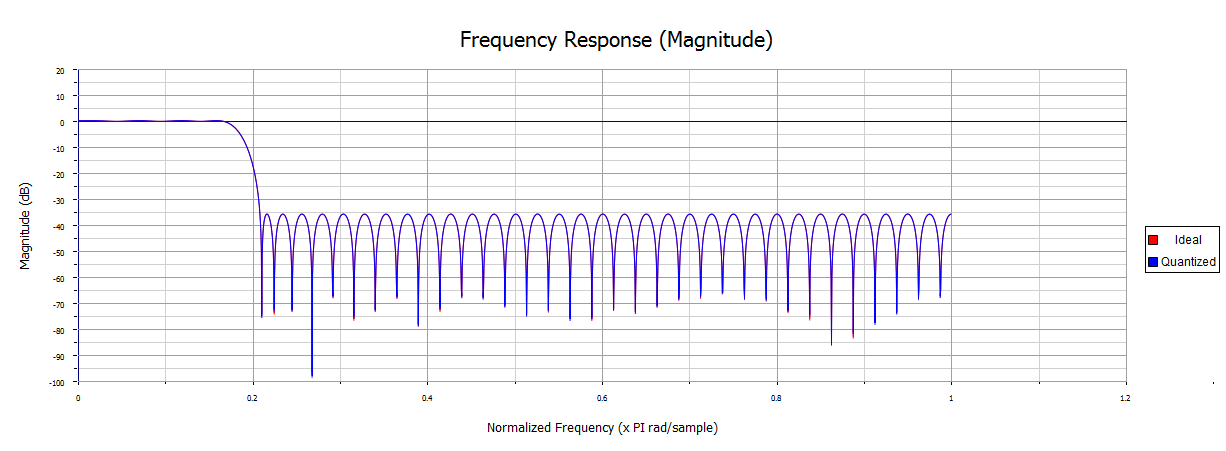
\includegraphics[width = 6.0in]{LowPass_Filter_Design.png}
	\caption{A low pass filter design.}
\end{figure}


 




